% Created 2014-02-19 三 21:48
\documentclass[11pt]{article}
\usepackage[utf8]{inputenc}
\usepackage[T1]{fontenc}
\usepackage{fixltx2e}
\usepackage{graphicx}
\usepackage{longtable}
\usepackage{float}
\usepackage{wrapfig}
\usepackage{rotating}
\usepackage[normalem]{ulem}
\usepackage{amsmath}
\usepackage{textcomp}
\usepackage{marvosym}
\usepackage{wasysym}
\usepackage{amssymb}
\usepackage{hyperref}
\tolerance=1000
\author{elvestar}
\date{\today}
\title{Minos Master 详细设计}
\hypersetup{
  pdfkeywords={},
  pdfsubject={},
  pdfcreator={Emacs 24.3.1 (Org mode 8.2.5h)}}
\begin{document}

\maketitle
\tableofcontents


\section{Master}
\label{sec-1}
\section{元信息管理}
\label{sec-2}
\subsection{元信息压缩}
\label{sec-2-1}
使用Snappy压缩。

\subsection{传输流Checkpoint的存储}
\label{sec-2-2}

之前传输流的Checkpoint是和日志配置一起存储在Zookeeper上面的,但是最近发现几份日志
的Checkpoint暴涨,超过ZK的1M限制,导致Master频繁出core。现在要寻求一种更好的存储
方式。

备选方案如下:
\begin{center}
\begin{tabular}{rlll}
序号 & 方案 & 优点 & 缺点\\
\hline
1 & HDFS & HDFS应用广泛,且能满足应用场景 & 需要依赖libhdfs和libjvm,且受集群可用性限制\\
2 & Mola & 上一个项目用Mola,效果很好,且应用场景完全匹配(KV) & Mola的Value大小有限制,是4M\\
3 & NFS & 通过fuse能像本地Filesystem一样来用NFS & NFS刚面世,稳定性还未知\\
4 & 本地Filesystem & 方便易用,且能满足易用场景 & 单机存储,受磁盘故障影响,故障迁移麻烦\\
\end{tabular}
\end{center}

决定本期先使用本地Filesystem存储,并以循环写入的方式为每个传输流存储多个版本的
Checkpoint。未来会考虑NFS,也可能继续用本地Filesystem,继续用的话就要作更多的容错
性考虑(可以研究下HDFS的元数据本地化存储方案)。

\subsubsection{Checkpoint本地化}
\label{sec-2-2-1}
目前,传输流的Checkpoint的存储是由MinosMeta来负责存储到ZK。升级为本地化存储之后,
需要在MinosMeta模块到本地Filesystem之间新加一层,相关类叫做
\textbf{LocalMetaDataAccessor} 。

LocalMetaDataAccessor会为每份日志维护多个版本的Checkpoint,这些Checkpoint的存储路
径如下:
\begin{verbatim}
/path/to/log-flow/${log_module_id}/${timestamp}
\end{verbatim}
其中,\$\{timestamp\}代表存储Checkpoint这个时刻的时间戳。

传输流Checkpoint的本地存储相关的过程有:
\begin{itemize}
\item 获取某日志的Checkpoint
\item 存储某日志的Checkpoint
\item 删除某日志的Checkpoint
\end{itemize}

\paragraph{多版本Checkpoint}
\label{sec-2-2-1-1}
多版本Checkpoint的的意义不仅在于存储多版本,还能提高容错性。当磁盘故障或其他故障
导致某个Checkpoint坏掉时,MinosMeta还能读取其他版本的Checkpoint并从中恢复。

默认情况下,会存储三个版本的Checkpoint,这个配置项是可以修改的(最小可以改成1)。
但是,这个配置项是针对整个Master,而不能针对某个传输流单独配置。本期Master不支持
为每个传输流配置Checkpoint存储的版本数的特性,因为这样做会增加复杂性,且没有明显
的收益。
\paragraph{获取某日志的Checkpoint}
\label{sec-2-2-1-2}
MinosMeta会根据传入的log\_module\_id拼装出该日志的Checkpoint的目录,如下:
\textbf{/path/to/log-flow/\$\{log\_module\_id\}} ,然后调用LocalMetaDataAccessor的
GetMetaData接口。

GetMetaData的过程如下:
\begin{enumerate}
\item 判断路径是否存在,不存在则返回false;
\item 获取路径下面的所有文件,如果文件数目为空,则返回false;
\item 通过文件名中的时间戳来为这些文件排序,选择第i个文件,读取内容返回给调用者;
\end{enumerate}

当调用者获取第i版本的Checkpoint之后,发现该Checkpoint不可用,则它会尝试调用第i+1版
本Checkpoint。如果所有版本的Checkpoint都不可用,则这个传输流就初始化失败。
\paragraph{存储某日志的Checkpoint}
\label{sec-2-2-1-3}
拼装Checkpoint存储目录仍然由MinosMeta负责,然后调用LocalMetaDataAccessor的
UpdateMetaData/AddMetaData接口。

UpdateMetaData/AddMetaData的过程如下:
\begin{enumerate}
\item 判断目录是否存在,不存在则创建目录;
\item 以当前时间戳作为文件名,在目录下创建文件,将Checkpoint存储到这个文件中。如果该
文件已经存在,则覆盖写;
\item 获取路径下面的所有文件,按照文件名中的时间戳排序。如果Checkpoint文件数目超过
Checkpoint版本的最大数目,则删除较老的Checkpoint文件;
\end{enumerate}
\paragraph{删除某日志的Checkpoint}
\label{sec-2-2-1-4}
拼装Checkpoint存储目录还是由MinosMeta负责,然后调用LocalMetaDataAccessor的
DeleteMetaData接口。

DeleteMetaData的过程如下:
\begin{enumerate}
\item 判断目录是否存在,不存在则返回false;
\item 递归删除该目录;
\end{enumerate}

\subsection{规模和限制}
\label{sec-2-3}
每个传输流的Checkpoint按照平均1M来算,存储三个版本,就是每个日志需要3M。每个
Master管理的

\section{传输流管理}
\label{sec-3}
\subsection{BNS同步}
\label{sec-3-1}
\subsection{为慢节点调用Fallback}
\label{sec-3-2}
\subsection{为MA选择MC}
\label{sec-3-3}

\section{Notifier}
\label{sec-4}
\subsection{通知模块的职责}
\label{sec-4-1}
Minos的通知模块的职责是在数据分片传输就位时,通知下游的数据系统该数据分片
(DataSlice)可用了。

拿通知云图(CloudAtlas)来说,通知模块具体职责包括:
\begin{enumerate}
\item 获取上次通知的时间点,以及通知间隔,获得一个有待通知的数据分片列表;
\item 判断待通知的数据分片是否传输就位;
\item 调用云图client的AddSlice接口,来对已就位的数据分片执行通知;
\item 当成功为某个数据分片执行通知后,保存通知进度;
\end{enumerate}
\subsection{模块过程}
\label{sec-4-2}
\subsubsection{为各个传输流调用通知接口}
\label{sec-4-2-1}
Monitor类 \textbf{定期轮询} 所有的传输流,并以传输流的当前Checkpoint(类型为
LogFlowMessage)作为参数,调用Notifier类的 \textbf{Notify()} 接口。
\subsubsection{获取传输流未通知的DataSlice}
\label{sec-4-2-2}
在Notifier的Notify()函数中,会
\subsubsection{判断数据分片是否准备就绪}
\label{sec-4-2-3}
通知模块有一个static的函数,专门用来判断某传输流的某数据分片是否已经就绪。函数原型如下:

\begin{verbatim}
static bool IsDataSliceReady(const LogFlowMessage& log_flow,
			     const DataSlice& data_slice);
\end{verbatim}
\subsubsection{执行通知}
\label{sec-4-2-4}
为了不阻塞调用线程,Notifier的Notifier()接口的工作其实只是讲DataSlice添加到
Notifier内部的通知队列中,然后立刻返回。有一个内部通知线程负责从通知队列中取
DataSlice,然后执行真正的通知下游的过程。
\subsubsection{通知成功后,将通知进度写回到传输流}
\label{sec-4-2-5}
内部通知线程为某DataSlice通知成功后,会主动将通知进度写回传输流,传输流会把通知进
度作为原信息定期保存起来。

Notifier会调用LogFlowManager的GetLogFlow()接口来获取DataSlice的LogFlow。LogFlow提
供了 \textbf{UpdateLatestNotifiedSlice()} 的接口,来供Notifier写回通知进度。
\subsection{通知条件}
\label{sec-4-3}
获取传输流中所有 \textbf{没有被disabled} 的节点的synced的log\_time列表,如果全部log\_time
均大于待通知的DataSlice的timestamp\_end,则认为可以通知,否则,不能通知。

\section{Alarmer}
\label{sec-5}
\subsection{报警模块的职责}
\label{sec-5-1}
\begin{itemize}
\item 判断传输流是否发生了需要报警的异常
\item 向指定用户或组发送短信报警和邮件报警
\end{itemize}
\subsection{主要过程}
\label{sec-5-2}
\begin{enumerate}
\item 判断传输流是否发生了异常
\item 根据预定义的报警策略,判断本次是否需要报警
\item 发报警
\end{enumerate}
\subsection{传输流状态与报警条件}
\label{sec-5-3}
Minos将数据传输到集群后,Master通过定期向下游计算系统执行 \textbf{通知} 来让下游使用这部
分数据。所以说, \textbf{通知进度} 是传输流状态的最主要的标记,也是Master进行报警的最主
要依据(目前是唯一依据。2014-02-12)
\subsection{短信报警}
\label{sec-5-4}
用户在新建Minos日志传输时,填写的是用户邮箱前缀(如zhongyi01),Master为了达成报
警,有两个难点:
\begin{enumerate}
\item 根据邮箱前缀来获取其对应的手机号
\item 在程序中向指定手机号发短信
\end{enumerate}

对于第一点,可以用公司提供了一个用soap实现的公共服务来实现。不过这会为Master引入
soap client。对于第二点,可以调用公司每台机器的gsmsend脚本。例子如下:
\begin{verbatim}
gsmsend -s emp01.baidu.com:15003 -s emp02.baidu.com:15003 18810001881@"I'm zhongyi"
\end{verbatim}

幸运的是,我们组的OP自己开发了一个专门的报警工具。我只需要向指定的数据库表insert一
条记录(包含邮箱前缀和报警内容),该报警工具就会触发报警。

\subsubsection{短信报警表的结构}
\label{sec-5-4-1}
\begin{verbatim}
mysql> desc t_alarm_info;
+-----------+----------------+------+-----+---------+-------+
| Field     | Type           | Null | Key | Default | Extra |
+-----------+----------------+------+-----+---------+-------+
| data_id   | bigint(20)     | NO   | PRI | NULL    |       |
| baseTime  | datetime       | NO   | PRI | NULL    |       |
| mail_to   | varchar(10240) | YES  |     | NULL    |       |
| mail_text | text           | YES  |     | NULL    |       |
| gsm_to    | varchar(10240) | YES  |     | NULL    |       |
| gsm_text  | text           | YES  |     | NULL    |       |
| sendTime  | datetime       | YES  |     | NULL    |       |
| is_send   | smallint(6)    | NO   | MUL | 0       |       |
+-----------+----------------+------+-----+---------+-------+
\end{verbatim}
\subsubsection{向表中插入记录以触发报警}
\label{sec-5-4-2}
向表中插入一条记录,就会触发报警。SQL语句如下:
\begin{verbatim}
insert into t_alarm_info (data_id, baseTime, gsm_to, gsm_text) values (7881, NOW(), "zhongyi01", "hehehehehe");
\end{verbatim}

data\_id对应于LDM中的logid\_id\_\_plan,如果是Minos的话,则对应于log\_module。由于
data\_id和baseTime共同构成了这种表的主键,所以两条记录这两个字段相同的话,第二条记
录将会插入失败。
\subsection{邮件报警}
\label{sec-5-5}

\subsection{报警逻辑抽取}
\label{sec-5-6}
\subsection{报警逻辑详细设计}
\label{sec-5-7}

\section{监控与统计}
\label{sec-6}
\subsection{全局counter}
\label{sec-6-1}
在Master内,维护者一批全局的Counter,通过监控这些Counter及其变化,可以监控系统的整体运行情况。

\begin{center}
\begin{tabular}{ll}
Counter & \\
\hline
节点更新状态的次数 & \\
对节点执行Fallback的次数 & \\
短信报警的次数 & \\
邮件报警的次数 & \\
 & \\
\end{tabular}
\end{center}
\section{线下环境}
\label{sec-7}
为线下Master的特殊配置:
\begin{center}
\begin{tabular}{ll}
配置项 & 值\\
\hline
FLAGS\_is\_offline & 设为true\\
CloudAtlas & 线下(在加好白名单之前,先禁掉)\\
旧DtMeta & 线下\\
LSP & 线下\\
集群 & QA线下集群\\
HDFS路径 & 规则不变\\
\end{tabular}
\end{center}
\section{多Master方案}
\label{sec-8}
\subsection{前期设想}
\label{sec-8-1}
\begin{enumerate}
\item 多个Master互作主备,放在一个BNS里面。
\item 每个Node启动时,根据BNS来随机找寻一个Master,询问它自己的log\_module\_id该被那个
Master管理。
\item 这些Master中有且只有一个Master为中央Master,当这个中央Master挂掉之后,这批
Master中会有一个Master自动升级为中央Master。
\item 中央Master主要负责Minos系统核心元数据(LogConfig)的管理,其他Master任务的分配,
以及各传输流信息的汇总。当然,中央Master也可以拥有传输流管理的功能。当中央
Master负载较轻或者系统只有一台Master时,中央Master也会承担传输流管理。
\end{enumerate}
\subsection{Zookeeper目录结构}
\label{sec-8-2}

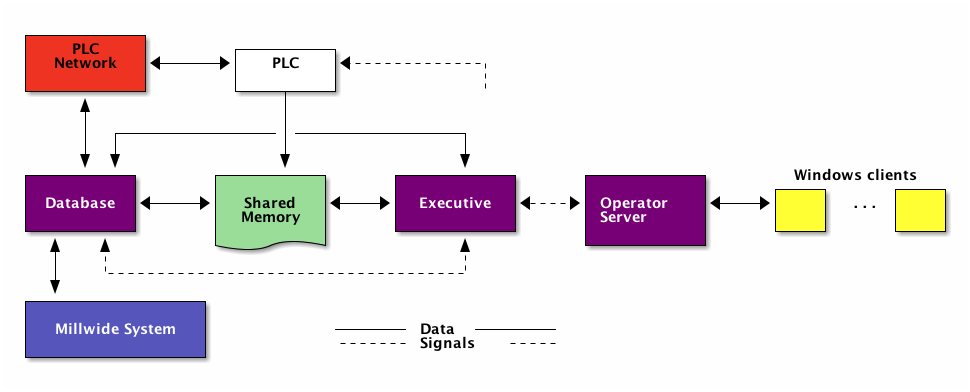
\includegraphics[width=.9\linewidth]{some_filename.png}

根节点
\begin{verbatim}
/minos
/minos/log-config
/minos/master
\end{verbatim}

log-config节点
\begin{verbatim}
/minos/log-config/1
/minos/log-config/2
\end{verbatim}

master节点
\begin{verbatim}
/minos/master/10.10.14.0
/minos/master/10.10.14.1
\end{verbatim}
\subsection{设计图}
\label{sec-8-3}

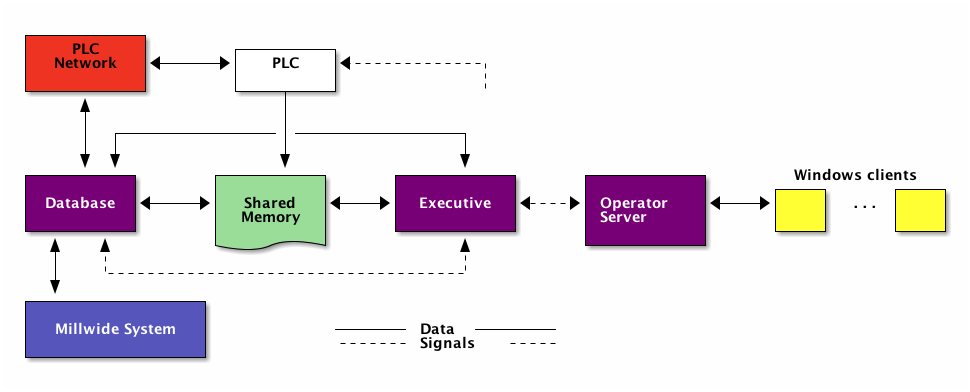
\includegraphics[width=.9\linewidth]{some_filename.png}
% Emacs 24.3.1 (Org mode 8.2.5h)
\end{document}
